\documentclass[../../main.tex]{subfiles}


\begin{document}
\subsection*{(a)}
We created the following OLAP Table:\\
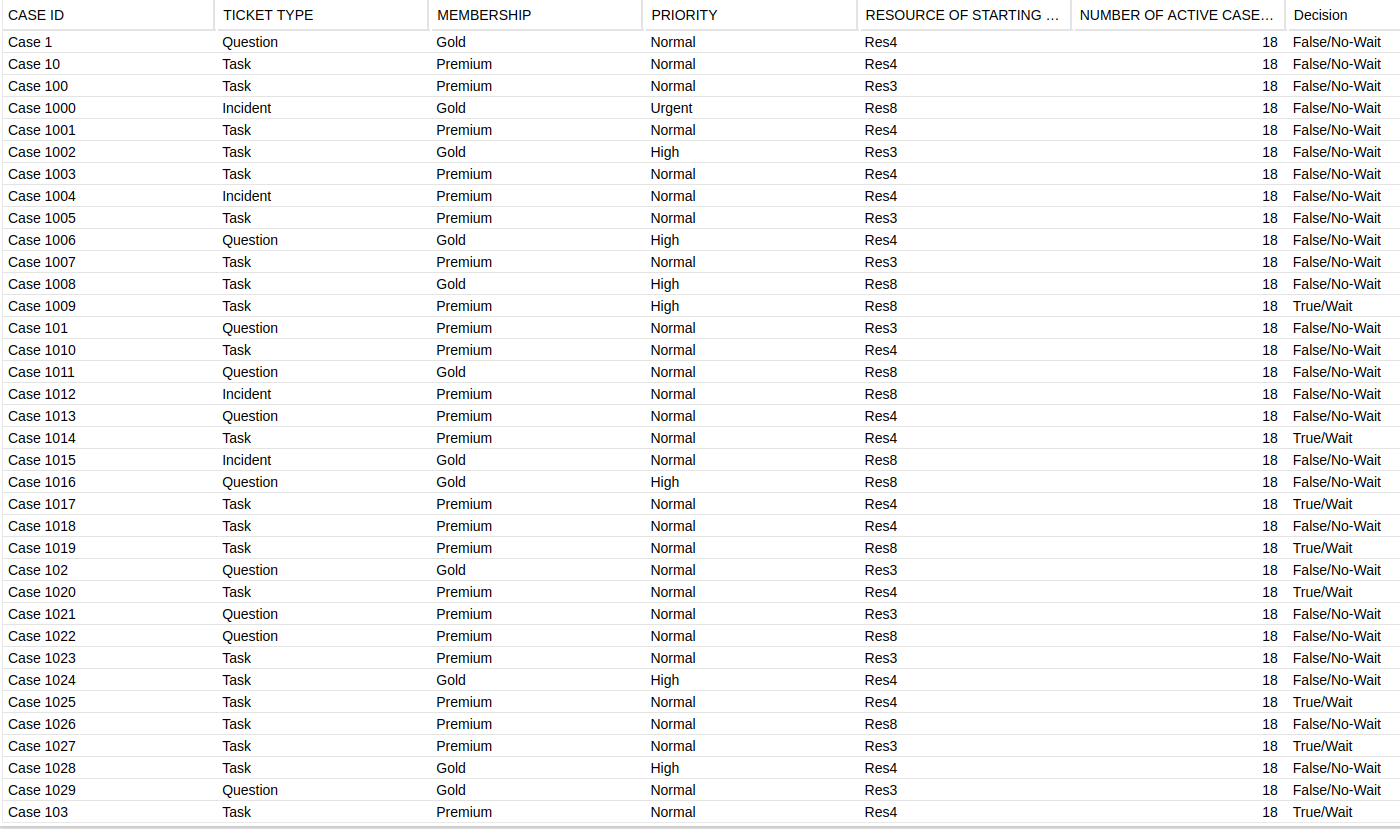
\includegraphics[width=\columnwidth]{img/Celonis_a_OLAP_Table.png}\\
For this, we used the following PQL Queries in the order of columns in the image left to right:
\begin{verbatim}
	"case_table_csv"."CASE ID"
\end{verbatim}
\begin{verbatim}
	"case_table_csv"."MEMBERSHIP"
\end{verbatim}
\begin{verbatim}
	"case_table_csv"."TICKET TYPE"
\end{verbatim}
\begin{verbatim}
	"event_table_csv"."PRIORITY"
\end{verbatim}
\begin{verbatim}
	PU_FIRST ( "case_table_csv", "event_table_csv"."RESOURCE")
\end{verbatim}
\begin{verbatim}
PU_FIRST("case_table_csv",
	RUNNING_SUM(
		CASE WHEN ACTIVITY_LAG("event_table_csv"."ACTIVITY") IS NULL
		THEN 1
		WHEN ACTIVITY_LEAD("event_table_csv"."ACTIVITY") IS NULL
		THEN -1
		ELSE 0
		END,
		ORDER BY ("event_table_csv"."TIMESTAMP")
	)
)
\end{verbatim}
\begin{verbatim}
CASE WHEN
	MATCH_PROCESS_REGEX ( "event_table_csv"."ACTIVITY", 'Wait' ) = 1 THEN 'True/Wait'
	ELSE 'False/No-Wait'
END
\end{verbatim}


\subsection*{(b)}
First, we export the OLAP Table and import it into RapidMiner as described in Instruction 2.\\
The resulting decision tree is evidently too large to fit into a PDF, thus we have added the description in the Appendix:\\
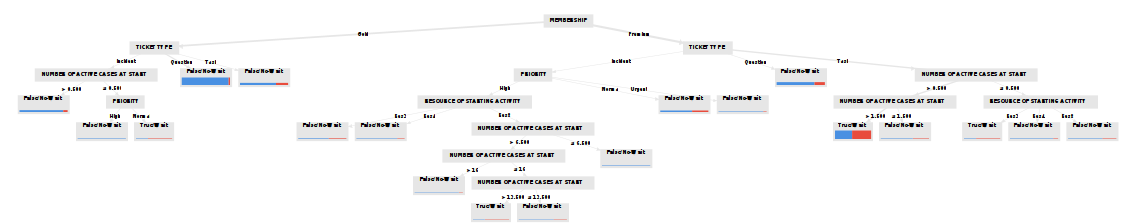
\includegraphics[width=\columnwidth]{img/RapidMiner_b_Decision_Tree.png}\\
We observed that only in extremely specific conditions cases are more likely to wait than not. In general, this depends largely on how many cases are already active in the beginning. This however varies depending on the Membership plan, what type of ticket the case is and priority the ticket is of. This would make sense, since more important issues to both the consumer and the company should be prioritized differently, thus resulting in these specific wait-conditions. Though it appears once in the tree, we do not believe that the resource has a significant influence in this.

After removing the attribute 'resource of starting activity', we get the same decision tree, pruned of the Resource-Split.

We can increase the minimal gain ratio to get a more simplified overview of the Decision Tree (see Appendix).\\
Here we see that tickets from Premium Memberships are more likely to be put on hold compared to tickets from Gold Memberships. However, this happens mostly at a large number of already running cases.

\end{document}
